\documentclass{beamer}
\usepackage{ctex, hyperref}
\usepackage[T1]{fontenc}

% other packages
\usepackage{latexsym,amsmath,xcolor,multicol,booktabs,calligra}
\usepackage{graphicx,pstricks,listings,stackengine}

\author{Genshin impact}
\title{原神}
\subtitle{课程报告}
\institute{提瓦特的大陆}
\date{1145年1月4日}
\usepackage{NJUPT}

% defs
\def\cmd#1{\texttt{\color{red}\footnotesize $\backslash$#1}}
\def\env#1{\texttt{\color{blue}\footnotesize #1}}
\definecolor{deepblue}{rgb}{0,0,0.5}
\definecolor{deepred}{rgb}{0.6,0,0}
\definecolor{deepgreen}{rgb}{0,0.5,0}
\definecolor{halfgray}{gray}{0.55}

\lstset{
    basicstyle=\ttfamily\small,
    keywordstyle=\bfseries\color{deepblue},
    emphstyle=\ttfamily\color{deepred},    % Custom highlighting style
    stringstyle=\color{deepgreen},
    numbers=left,
    numberstyle=\small\color{halfgray},
    rulesepcolor=\color{red!20!green!20!blue!20},
    frame=shadowbox,
}


\begin{document}

\kaishu
\begin{frame}
    \titlepage
    \begin{figure}[htpb]
        \begin{center}
            
\includegraphics[width=0.2\linewidth]{pic/swust.png}
        \end{center}
    \end{figure}
\end{frame}

\begin{frame}
    \tableofcontents[sectionstyle=show,subsectionstyle=show/shaded/hide,subsubsectionstyle=show/shaded/hide]
\end{frame}


\section{超导简介}

\begin{frame}{什么是超导?}
    \begin{itemize}[<+-| alert@+>] % 当然,除了alert,手动在里面插 \pause 也行
        \item “超导”是一种特殊的物理现象,指的是某些物质在低温条件下,电阻突然消失,变为零电阻的状态。这种现象称为超导电性,具备这种特性的材料称为超导体。在超导状态下,电流可以在不受任何电阻阻碍的情况下流动,因此可以在不过热或耗费大量能源的情况下创造超强磁场。同时,超导态还表现出完全抗磁性。但超导态必须在一定的温度、磁场和电流密度等临界参量范围内才能维持,一旦超越这些临界参量,超导态就会被破坏,恢复为有电阻的状态。
    \end{itemize}
\end{frame}


\section{石墨烯简介}

\subsection{什么是石墨烯}

\begin{frame}
    \begin{itemize}
        \item 石墨烯是一种由碳原子以sp$^2$杂化轨道组成六角型呈蜂巢晶格的二维碳纳米材料。石墨烯具有优异的光学、电学、力学特性,在材料学、微纳加工、能源、生物医学和药物传递等方面具有重要的应用前景,被认为是一种未来革命性的材料。
        \item 石墨烯(Graphene)是一种由碳原子以sp$^2$杂化方式形成的蜂窝状平面薄膜,是一种只有一个原子层厚度的准二维材料,所以又叫做单原子层石墨。它的厚度大约为0.335nm,根据制备方式的不同而存在不同的起伏,通常在垂直方向的高度大约1nm左右,水平方向宽度大约10nm到25nm,是除金刚石以外所有碳晶体(零维富勒烯,一维碳纳米管,三维体向石墨)的基本结构单元。另外,石墨烯几乎是完全透明的,另一方面,它非常致密,即使是最小的气体分子(氦气)也无法穿透。这些特征使得它非常适合作为透明电子产品的原料,如透明的触摸显示屏、发光板和太阳能电池板。作为目前发现的最薄、强度最大、导电导热性能最强的一种新型纳米材料,石墨烯被称为“黑金”,是“新材料之王”。
    \end{itemize}
\end{frame}

\subsection{石墨烯为什么会获得诺贝尔奖?}
\begin{frame}{是因为石墨烯真的很有用吗?}
    \begin{itemize}
        \item 统计物理中的Mermin-Wagner定理:任何具有连续对称性的二维热力学系统,在非零温下,其连续对称性不可能发生自发破缺。在得到这个定理之后,物理学家一般不对找到二维晶格抱有期待。即便我们可以说现实中没有完全严格的二维系统,大家也一般会说,这个条件放松了,最多也就是定理对应的非零温这个条件放松一点。大概在相当低的温度下可能找到准二维晶格——但意想不到的是,室温下就能找到石墨烯这种东西。
        \item 提供一种观点:“石墨烯拿到了诺贝尔奖,不是因为它有什么什么用,而是因为它对这个定理的“违背”,让人们震惊,而石墨烯本身,很可能并不比其他新发现的材料更有用。” —————北京大学田光善

    \end{itemize}
\end{frame}

\section{转角二维石墨烯}

\subsection{什么是转角}

\begin{frame}{什么是转角}
    \begin{itemize}
        \item 转角(Twist):当两片石墨烯以特定角度堆叠到一起时就会出现一些类似高温超导体的神奇特性。
        \item 将两套网格叠在一起并旋转一个角度就能产生称为莫尔条纹(moiré fringes)的干涉图案。在过去几年中,科学家们已经开始通过旋转单原子厚度的材料(如碳原子构成的二维蜂窝状晶格,也就是石墨烯)在原子尺度上实现和设计莫尔条纹。在2018年的两篇工作中,研究人员发现当两片石墨烯之间的转角达到约1度时,整个系统的物理性质会发生急剧的变化,变得类似于高温超导体。
    \end{itemize}
\end{frame}

\subsection{魔角石墨烯}
\begin{frame}{基本定义}
 	\begin{minipage}{0.5\textwidth}
		\begin{figure}
			\centering
			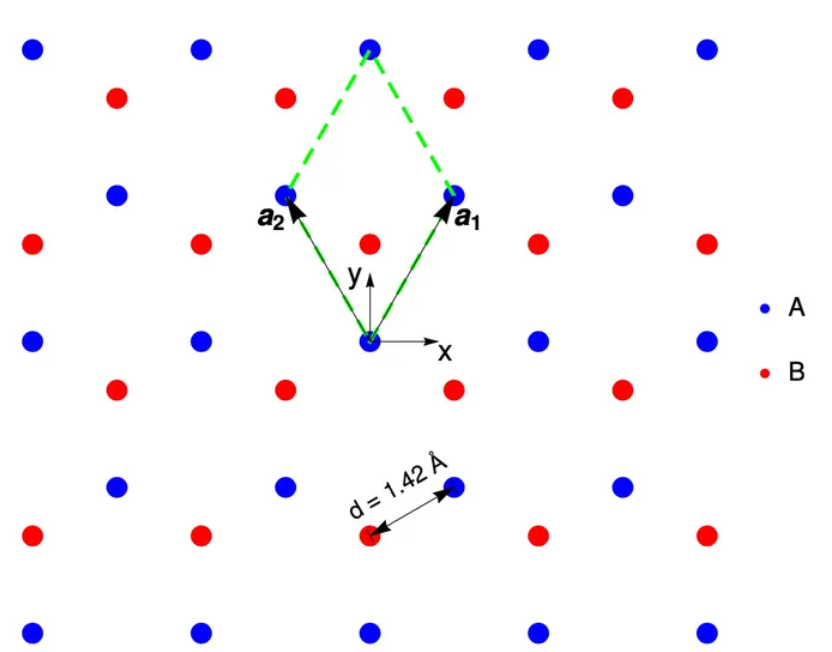
\includegraphics[width=\textwidth]{pic/gra.png}
		\end{figure}
	\end{minipage}%
	\begin{minipage}{0.5\textwidth}
		\begin{figure}
			\centering
			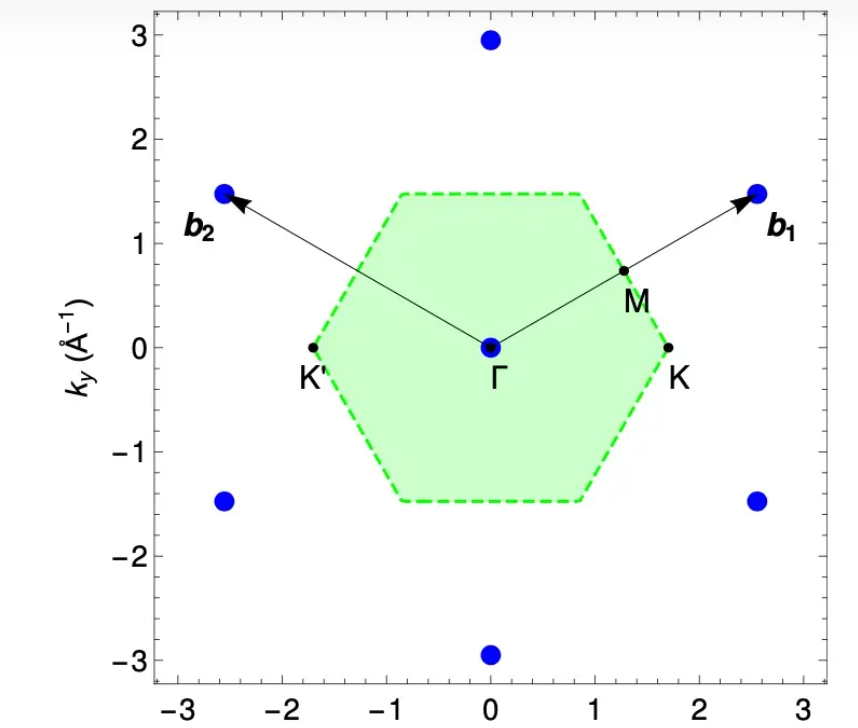
\includegraphics[width=\textwidth]{pic/grar.png}
		\end{figure}
	\end{minipage}
\end{frame}

\begin{frame}{理论推导与实验观测}
    \begin{exampleblock}{转角石墨烯平带条件\footnote{参考Bistritzer, R.,  MacDonald, A. H. (2011). Moiré bands in twisted double-layer graphene.Proceedings of the National Academy of Sciences,108(30), 12233-12237.}} % 加 * 
        \begin{equation*}
            \hbar v_f '=[1+3(\omega_0 ^2 +\omega_1 ^2)]^{-1}(1-3\omega_1 ^2)\hbar v_f=0
        \end{equation*}
    \end{exampleblock}
    \begin{exampleblock}{代入参数计算}
     \begin{equation*}
     \omega_1=\frac{1}{\sqrt{3}},2\sin{\frac{\theta}{2}}\approx \theta,\theta_{magic}=0.0188rad \approx 1.1^\circ
        \end{equation*}
    \end{exampleblock}
\end{frame}

\begin{frame}
   单层石墨烯的许多性质都可以用自由电子的物理图像来定性地理解,在这个物理图像中电子之间的排斥作用被忽略掉了。例如,单层石墨烯中电子能量和动量的色散关系可以很好地近似为不依赖于周围电子的密度。“魔角”双层石墨烯的情况则截然不同(最大魔角大概为1度)。在这种情况下,电子会占据平带(平带也就是很平的能带)。由于这些平带的带宽很小,电子之间的相互作用不能再当做微扰来处理,这时候系统的物理性质就会强烈依赖于电子密度。这种强相互作用甚至会引起单层石墨烯中没有的物相:在特定的电子密度下,虽然在自由电子物理图像中系统应该是金属,但是实际系统表现为绝缘体;并且,就像高温超导体一样,这时候增加或减少电子密度会减小电阻并出现超导(电阻为零)。
\end{frame}


\begin{frame}{实验观测}
    \begin{figure}[htpb]
        \centering
        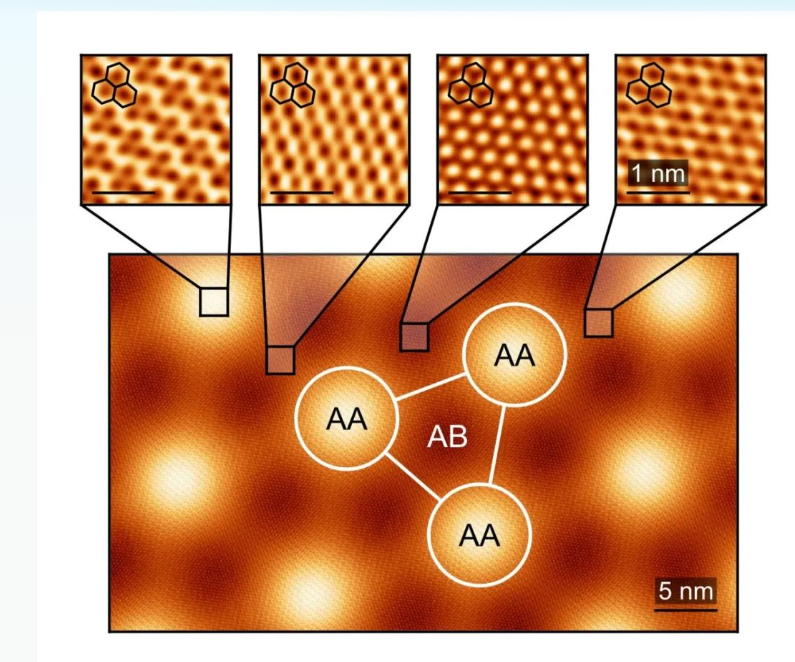
\includegraphics[width=0.5\linewidth]{pic/sm.png}
        
        \caption{扭曲双层石墨烯的扫描隧道显微镜图像}
    \end{figure}
\end{frame}

\begin{frame}
 \begin{itemize}
        \item 普林斯顿大学领导的一个科学家团队对精确的微观基础进行了成像,这些基础负责在一种称为魔角扭曲双层石墨烯(MATBG)的材料中观察到的许多量子相。这种非凡的材料由以二维六边形图案排列的碳原子扭曲层组成,近年来一直处于物理学研究的前沿,特别是在凝聚态物理学中。研究人员首次能够专门捕获相互作用电子的微观行为的前所未有的精确可视化,这些相互作用电子产生了MATBG的绝缘量子相。此外,通过使用新颖和创新的理论技术,他们能够解释和理解这些行为。他们的研究发表在《自然》杂志上。扭曲双层石墨烯的惊人特性于2018年由麻省理工学院(MIT)的Pablo Jarillo-Herrero及其团队首次发现。他们表明这种材料可以是超导的,一种电子在没有任何阻力的情况下自由流动的状态。这种状态对我们的许多日常电子产品至关重要,包括用于MRI和粒子加速器的磁铁,以及用于构建量子计算机的量子比特(称为量子比特)的制造。
    \end{itemize}    
\end{frame}

\section{理论计算}
\begin{frame}{理论计算结果}
    \begin{figure}[htpb]
        \centering
        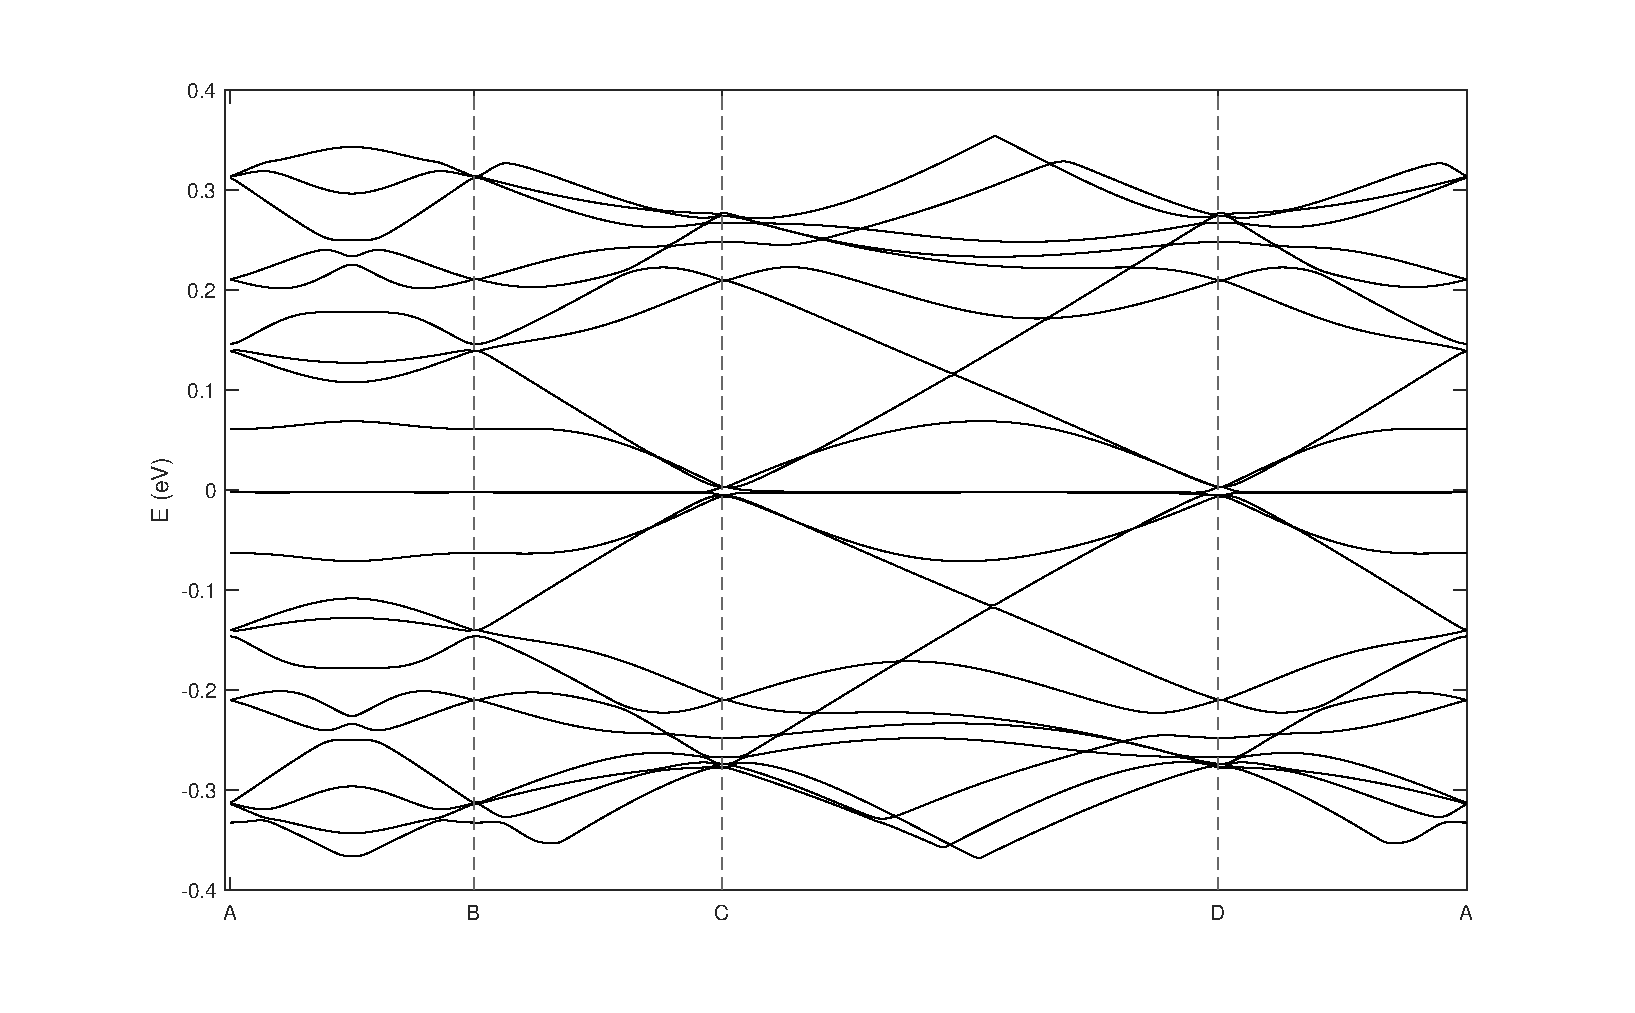
\includegraphics[width=0.8\linewidth]{pic/untitled.eps}
        
        \caption{计算得到的平带}
    \end{figure}
\end{frame}
\begin{frame}{理论计算结果}
    \begin{figure}[htpb]
        \centering
        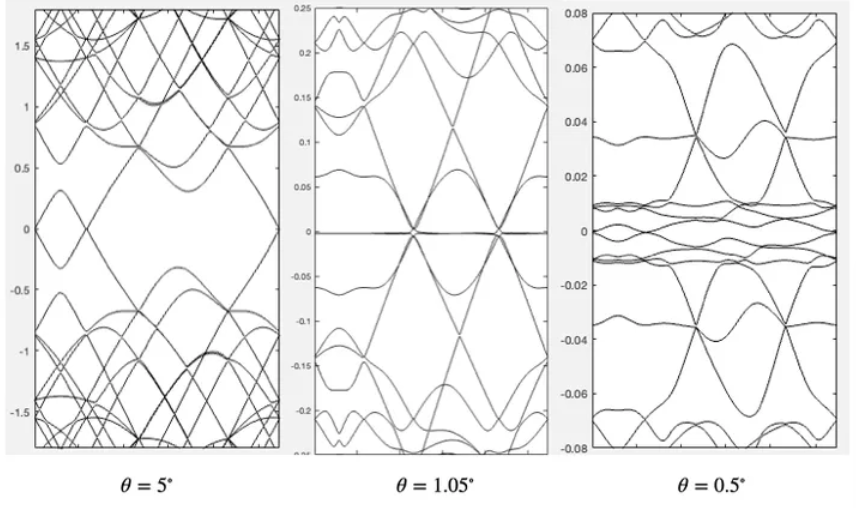
\includegraphics[width=0.8\linewidth]{pic/pd.png}
        
        \caption{$\theta=1.05^{\circ}$时观察到平带}
    \end{figure}
\end{frame}


\begin{frame}
    \begin{center}
        {\Huge\calligra Thanks!}
    \end{center}
\end{frame}

\end{document}